% !TEX program = xelatex
\documentclass[14pt]{beamer}
\usepackage{pyconuk2015}

\mode<presentation>
{
  \usetheme{default}
}

\title{Leadership of Technical Teams}
\author{Owen Campbell}
\date[PyCon UK 2015]{
  @opcampbell\\
  \vspace{1cm}
  18th September, 2015\\
  PyCon UK, Coventry}

\begin{document}

\begin{frame}
  \titlepage{}
  \speakernote{
    ?         get rid of help\textCR
    F5        full screen\textCR
    spacebar  start timer
  }
\end{frame}

{
  \begin{frame}<beamer>{Outline}
    \tableofcontents
    \speakernote{
      Not a definitive guide
    }
  \end{frame}
}

  \section{Introduction}

    \blankscreen{
      Judge whether to stay\
    }

    \begin{frame}{}
      \begin{columns}
        \column{0.4\textwidth}
          \includegraphics[scale=0.1]{images/zx81}
          \speakernote{
            35 years coding experience\textCR
            Too young for the ZX80, too old for the Spectrum\textCR
          }
        \pause
        \column{0.3\textwidth}
          
\includegraphics[scale=0.1]{images/ici}\\[2em]
          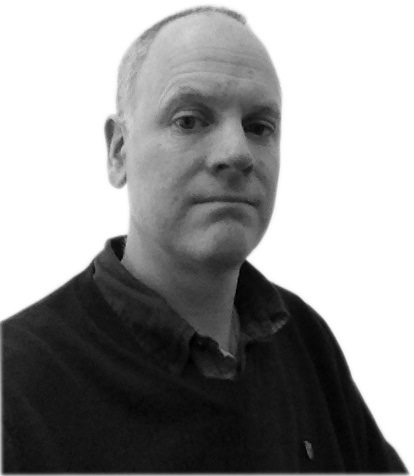
\includegraphics[scale=0.17]{images/owencampbell}
          \speakernote{
            \textCR
            Hedge Funds to Hospitals to Housing Associations\textCR
            One more thing to say about myself....\textCR
          }
        \pause
        \column{0.3\textwidth}
          
\includegraphics[scale=0.25]{images/scouts}
          \speakernote{
            \textCR
            ** Practice makes perfect **
          }
      \end{columns}
    \end{frame}

  \section{Authority}
    \blankscreen{}

    \begin{frame}{}
      \begin{Huge}
        \faHeart \hfill
        \pause
        \faHandGrabO \hfill
        \pause
        \faSignOut
        \pause
        \speakernote{
          Don't pick a fight that's not necessary but don't shy away from one that is\textCR
          \textCR
          ** Schooze 'em, Bruise 'em or Lose 'em **
        }
      \end{Huge}\\
      \vfill
      \begin{center}\large "Schmooze 'em, bruise 'em or lose 'em"\end{center}
    \end{frame}

  \section{Priorities}
    \blankscreen{}

    \begin{frame}{}
      % Comment to allow building from within this file
%!TEX root = pyconuk2015.tex

\tikzstyle{item} = [decorate, ellipse, line width=0.4mm, draw=blue, minimum height=14mm]
\tikzstyle{line} = [line width=0.5mm]

\begin{center}
    \HumorSans
    \resizebox{10cm}{!}{
        \begin{tikzpicture}[decoration=freehand]
            \node (team) [item, circle, draw=red] at (0, 0) {Team};
            \pause
            \node (customers) [item] at (90:3) {Customers};
            \freedraw [line](team) -- (customers);
            \pause
            \node (investors) [item] at (20:4) {Investors};
            \freedraw [line](team) -- (investors);
            \pause
            \node (others) [item] at (340:4) {Other Teams};
            \freedraw [line](team) -- (others);
            \pause
            \node (process) [item] at (270:3) {Process};
            \freedraw [line](team) -- (process);
            \pause
            \node (resources) [item] at (200:4) {Resources};
            \freedraw [line](team) -- (resources);
            \pause
            \node (deliverables) [item] at (160:4) {Deliverables};
            \freedraw [line](team) -- (deliverables);
        \end{tikzpicture}
    }
\end{center}

      \speakernote{
        Your items may be different\textCR
        Mind map seems to work better than checklists\textCR
        \textCR
        ** Expect the Unexpected **
      }
    \end{frame}

  \section{Style}

    \begin{frame}{Leadership Styles}
      \begin{itemize}
        \item Dictatorial
        \item Paternalistic
        \item Consensual
        \item Democratic
        \item Hands Off
      \end{itemize}
    \end{frame}

    \begin{frame}{Style vs. Expertise}
      % Comment to allow building from within this file
%!TEX root = pyconuk2015.tex

\tikzstyle{axis} = [line width=0.5mm]
\tikzstyle{sweetspot} = [
    decorate, ellipse, rotate=45, line width=0.5mm, draw=green,
    fill=green, opacity=0.2,
    minimum width=80mm, minimum height=10mm]
\tikzstyle{danger} = [
    decorate, circle, line width=0.5mm, draw=red,
    fill=red, opacity=0.2, font=\small, text opacity=1,
    minimum width=28mm]

\begin{center}
    \HumorSans
    \begin{tikzpicture}[decoration=freehand]
        \freedraw [axis] (0, -3) -- (0, 3);
        \freedraw [axis] (-3, 0) -- (3, 0);
        \node at (-4, 0) {Rookie};
        \node at (4, 0) {Guru};
        \node at (0, 3.5) {Dictator};
        \node at (0, -3.5) {Observer};
        \pause

        \node [sweetspot] at (0, 0) {};
        \pause
        \node [danger] at (-1.5, 1.5) {Git};
        \pause
        \node [danger] at (1.5, -1.5) {Subversion};
    \end{tikzpicture}
\end{center}

      \speakernote{
        ** One notch at a time **
      }
    \end{frame}

  \section{Process}
    \blankscreen{}
    \begin{frame}{\large Manifesto for Agile Software Development}

      {\footnotesize \color{black} We are uncovering better ways of developing
      software by doing it and helping others do it.
      Through this work we have come to value:}
      \vfill
      \tikzmarkin<2->{a1}
      \begin{description}
        \begin{small}
          \item [Individuals and interactions] over processes and tools\tikzmarkend{a1}
          \item [Working software] over comprehensive documentation
          \item [Customer collaboration] over contract negotiation
          \item [Responding to change] over following a plan
        \end{small}
      \end{description}
      \vfill
      {\footnotesize That is, while there is value in the items on
      the right, we value the items on the left more.}

      \begin{block}{}
        {\tiny
          Kent Beck\hspace{5pt}
          Mike Beedle\hspace{5pt}
          Arie van Bennekum\hspace{5pt}
          Alistair Cockburn\hspace{5pt}
          Ward Cunningham\hspace{5pt}
          Martin Fowler\hspace{5pt}
          James Grenning\hspace{5pt}
          Jim Highsmith\hspace{5pt}
          Andrew Hunt\hspace{5pt}
          Ron Jeffries\hspace{5pt}
          Jon Kern\hspace{5pt}
          Brian Marick\hspace{5pt}
          Robert C. Martin\hspace{5pt}
          Steve Mellor\hspace{5pt}
          Ken Schwaber\hspace{5pt}
          Jeff Sutherland\hspace{5pt}
          Dave Thomas\\
          © 2001, the above authors
          this declaration may be freely copied in any form, but only in its entirety through this notice.}
      \end{block}

      \speakernote{
        ** Don't be a Git **
      }
    \end{frame}

  \section*{Summary}
    \blankscreen{}

    \begin{frame}{Summary}
      \begin{description}
        \item [Me] Practice Makes Perfect
        \pause
        \item [Authority] Schmooze, Bruise or Lose
        \pause
        \item [Priorities] Expect the Unexpected
        \pause
        \item [Style] One Notch at a Time
        \pause
        \item [Process] Don't be a Git
      \end{description}
    \end{frame}

    \begin{frame}{}
      \begin{description}
        \item [Twitter] @opcampbell
        \item [Google+] OwenCampbell1
        \item [Github] meatballs
      \end{description}
      \vfill
      \begin{description}
        \item [Slides] {\small owencampbell.me.uk/docs/pyconuk2015.pdf}
        \item [Source] {\small github.com/meatballs/pyconuk2015}
      \end{description}
    \end{frame}

\end{document}
